%++++++++++++++++++++++++++++++++++++++++
% Don't modify this section unless you know what you're doing!
\documentclass[letterpaper,12pt]{article}
\usepackage{tabularx} % extra features for tabular environment
\usepackage{amsmath}  % improve math presentation
\usepackage{graphicx} % takes care of graphic including machinery
\usepackage[margin=1in,letterpaper]{geometry} % decreases margins
\usepackage{cite} % takes care of citations
\usepackage[final]{hyperref} % adds hyper links inside the generated pdf file
\usepackage{listings}
\usepackage{csvsimple}
\usepackage{graphicx} % Allows including images
\hypersetup{
	colorlinks=true,       % false: boxed links; true: colored links
	linkcolor=blue,        % color of internal links
	citecolor=blue,        % color of links to bibliography
	filecolor=magenta,     % color of file links
	urlcolor=blue         
}
%++++++++++++++++++++++++++++++++++++++++
\begin{document}
\title{PyLab - Ohm and Power laws}
\author{Fredrik Dahl Bråten, Pankaj Patil}
\date{\today}
\maketitle

\section*{Exercise 1:  Introduction to fitting methods}

\section{Procedures}

\csvautotabular{../100k.csv}

\section{Analysis}

\begin{center}
    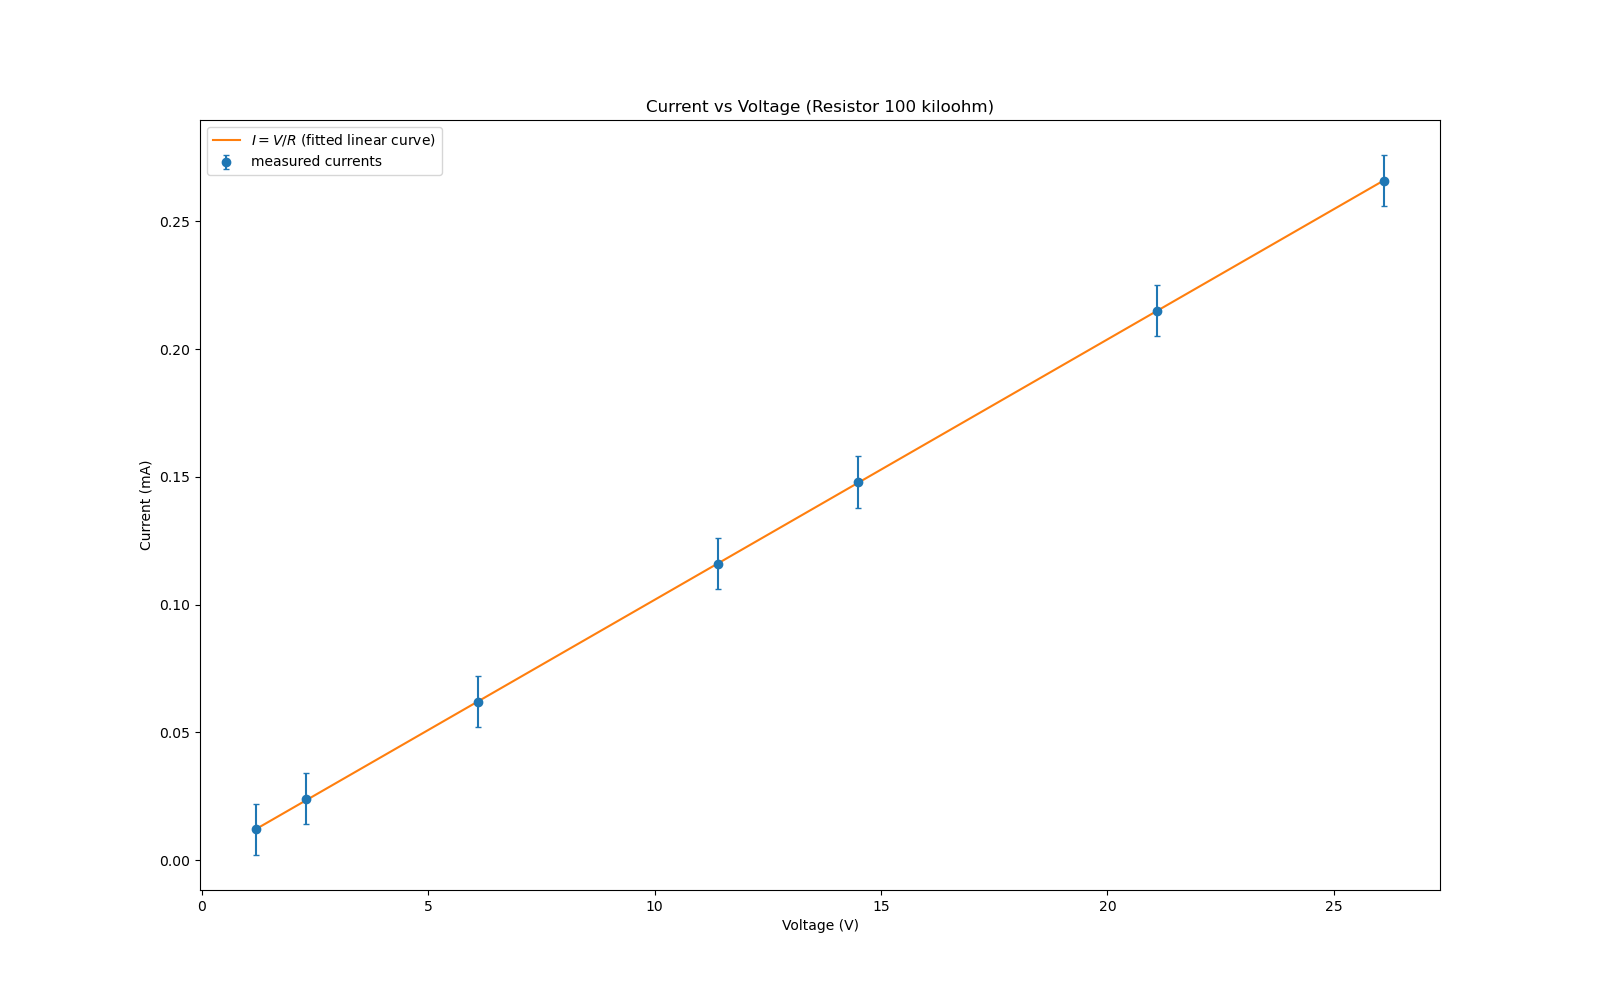
\includegraphics[width=1.0\linewidth]{../lab_1_ex_1_plot.png}    
\end{center}

\section{Conclusions}

\pagebreak

\section*{Exercise 3:  Nonlinear fitting methods II}

\pagebreak

\begin{center}
  \section*{Appendix}
\end{center}

\section*{Python Code: Exercise 1}

\lstinputlisting[language=Python]{../lab_1_ex_1_code.py}

\pagebreak

\section*{Python Code: Exercise 3}

\lstinputlisting[language=Python]{../lab_1_ex_1_code.py}

\pagebreak

\begin{thebibliography}{99}

\bibitem{melissinos}

\end{thebibliography}

\end{document}